%!TEX program = xelatex

\documentclass{HustGraduPaper}
\title{移动网络数据挖掘的研究与应用}
\author{徐聪}
\date{\today}
\school{电子信息与通信学院}
\classnum{通信1403班}
\stunum{U201413500}
\instructor{王邦}

\begin{document}
    \maketitle
    \statement
    \clearpage
    \pagenumbering{Roman}

    \begin{cnabstract}{移动网络;数据挖掘;统计分析}
        这里是摘要内容。
    \end{cnabstract}
    \begin{enabstract}{Mobile network;Data mining;statistic analysis}
        Here is the content of abstract.
    \end{enabstract}

    \tableofcontents
    \clearpage
    \pagenumbering{arabic}

    \section{绪论}
    
    \subsection{选题背景与意义}

    随着我国进入经济社会高速发展的阶段,电信行业也得到了快速的发展。从上世纪九十年代的
    2G发展落后于世界;到本世纪初3G时代,由我国大唐电信主导提出的TD-SCDMA标准被ITU确立成为3G主流
    制式;进入4G时代后,我国发展时间轴基本与世界先进水平国家保持同步,由我国主导的 TDD 通信制式
    将成为 5G 主流制式。到了 5G时代,我国主动成立 IMT-2020 推进组,举全产业链之力,
    积极推进 5G 技术标准发展,有望实现技术与市场双引领。
    
    除了传统通信的2、3、4G通信网络,中国的电信运营商也在顺应移动互联网发展趋势,
    发展出了诸如IPTV、窄带物联网(NB-IoT)、集客等新兴业务。以一个三线城市市级运营商来说,
    其网络管理中心负责主要业务包含无线及有线总共十二类业务,支撑十二类业务的背后包含十三类网络、四大类设备。
    如此众多的业务伴随而来的是海量的数据:日志、参数、拓扑等等。

    面对如此海量的数据,网络维护管理人员的维护难度也在不断攀升。传统的电信网络维护管理方式通常是以人工管理为主,
    运营商会向提供技术支持的公司雇佣代维人员对网络进行代理维护,而运营商内部人员则注重于对网络的管理以及自身核心业务,
    这种代维模式最初是为了解决网络规模扩张、运营商间的竞争压力不断增大的问题。但随着数据网络规模的进一步扩大,网络复杂性呈
    指数型上升,但是代维人员规模却不可能同步增加。除此之外,由于代维行业没有统一的行业标准,会出现代维人员业务水平参差不齐
    的情况,且在日常维护工作中仍采取较为传统的手段,导致运营商对于网络的管理维护并没有跟上网络快速发展的步伐,传统的维护
    模式已经不能适应将来的需求。

    近年来,随着计算能力的提升以及信息技术的发展,大数据的概念在运营商对网络管理维护中得到了广泛传播,将大数据以及数据挖掘的技术
    引入对于电信网络的运维管理来说是解决当前及未来需求的一种手段。由于运营商天生的特性,导致了它在数据规模这一块拥有
    天然的优势,而当前运营商的问题也是由于数据量过于巨大,而自身管理手段跟不上增长速度,导致的运维管理难度上升,
    而大数据及数据挖掘技术的引入会将这一劣势变为优势,不仅能解决当前数据量过大无法处理的难题,还能在此基础上对整个网络的流量、设备以及业务进行集中管控、统一编排。
    同时近年随着人工智能概念的火爆,一定程度上也是基于大数据及数据挖掘技术的成熟,因此在对电信网络数据进行大数据管理以及数据挖掘的基础上可以在合适的场景引入
    人工智能的方法,实现面向未来的智能运维。
    
    综上所述,基于移动通信网络的数据挖掘对于提升整个电信网络运维管理效率及质量具有较为实际以及深远的意义。在实际研究过程中,对运营商而言,
    大数据意味着对数据的获取、存储、分析、呈现等方式都提出了新的挑战,因此,如何对传统运维方式的这几个方面进行革新成为了运用大数据管理网络
    关键点。运营商希望将复杂的网络进行高效的管理,对于提升用户感知、网络优化、网络规划等多方面都具有实际的意义。\\
    \begin{generalfig}[htb]{大数据信息处理框架}{fig:frame}
		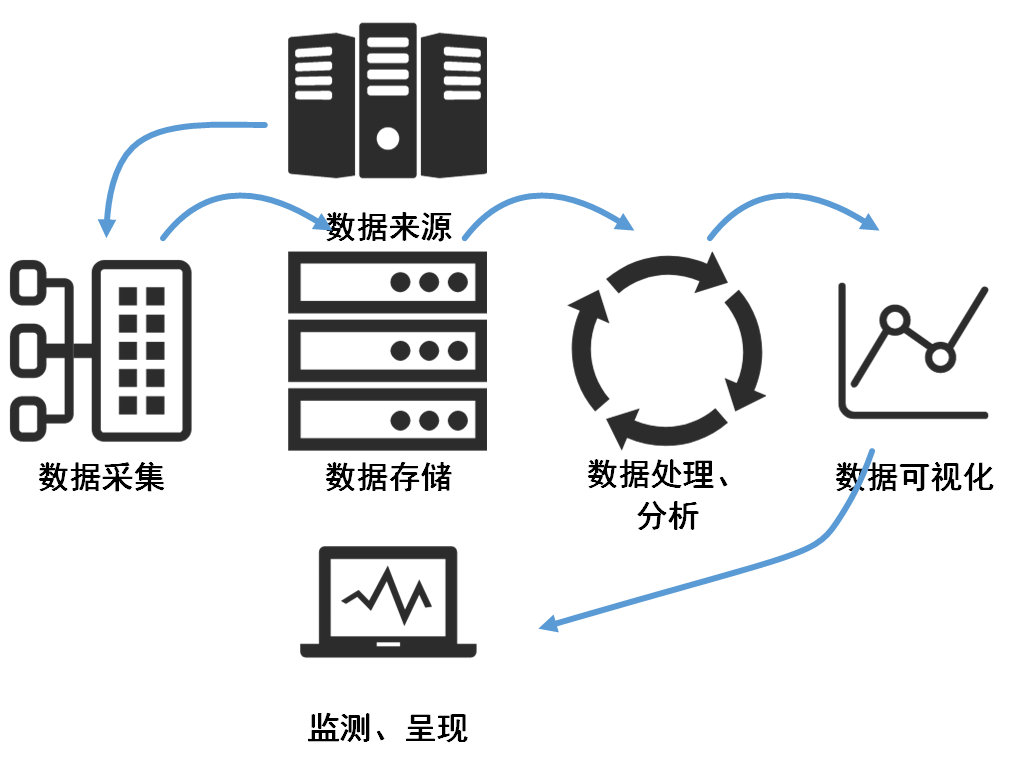
\includegraphics[width=\textwidth,scale = 0.5]{Figures/frame.png}
	\end{generalfig}

    \subsection{论文内容与成果}

    本文就数据挖掘技术在运营商网络管理和分析中的应用展开探索性讨论,从运营商现状出发,结合实际情况以及运维中的痛点进行分析,利用大数据及数据
    挖掘的方法探索运营商面临的海量数据采集及处理问题,同时还在数据分析方面进行了初步的尝试。主要包括了对大数据应用的数据采集、数据分析、以及
    数据呈现三个部分。

    第一部分就当前运营商面临的多系统数据采集的难点进行探索解决,由于运营商对网络情况感知的实时性要求较高,因此数据采集采用主动监控的方式采集数据,
    通过主动监控采集数据后对数据进行预处理及存储,为上层的分析和应用提供数据基础。针对运营商的多系统多数据源这一现状这里采用了区别于传统采集手段的分布式采集系统。

    第二部分在采集模块采集预处理存储后的数据基础上进行分析,从价值密度较低的数据中挖掘出对运营商网络管理有利的结论或建议。具体来说,本文就4G网络投诉问题进行了建模以及
    分析溯源,然后给出了网络优化的分析建议。

    最后,第三部分的数据呈现部分我们采用了丰富的图表形式来对数据分析结果进行直观有效的展示,使得网络管理运维人员能够更加便捷的了解
    网络情况,对网络问题及时做出应对。

    \subsection{论文结构}

    第一章绪论,主要介绍论文的选题背景以及研究意义,介绍了当前运营商在网络管理维护工作中的窘境,以及大数据及数据挖掘技术在相关工作中
    的作用以及意义。随后对本文所作的工作进行了简要的介绍,并从数据挖掘技术的应用的三个步骤进行了概括阐述。最后介绍了本篇文章的组织架构。

    第二章相关知识综述,对运营商的网络现状进行了介绍,介绍了运营商的网络数据管理现状;还对数据挖掘应用相关技术进行了概述,包括了数据采集手段以及数据呈现方式,
    为实际的探索应用确立了思路与基础。

    第三章为移动网络数据挖掘应用的设计与实现,包括对系统的需求分析以及具体技术的应用及实现方式,包括了数据采集、数据分析以及最后对分析结果的呈现。本章还就
    投诉问题为例进行了较为深层的分析。

    第四章为总结与展望,主要对本文所作工作进行总结,总结本文的创新点以及在实际应用中的意义,同时指出设计上的不足,为未来的工作方向做出展望。

    \clearpage
    \section{相关知识综述}
    \subsection{运营商网络运维现状介绍}

    现在是一个数据化的时代,也是一个移动化的时代。著名分析公司Gartner在报告中指出未来的公司都将是数据公司,现代人生活中被各种移动应用所环绕,移动网络流量
    出现井喷式的增长。作为网络运营商来说,爆炸增长的数据流量意味着网络管理维护难度的升级,更为甚者,如何避免自己在移动网络时代边缘化而仅仅成为移动应用的通道,
    都是当前时代环境下运营商所面临的挑战。但随着大数据及数据挖掘技术的成熟,上文所提到的挑战也可以转化为运营商转型升级的机遇,因此如何在保证自己服务质量的同时,
    发挥天然具有的流量数据优势,无论是从海量的日志数据中分析出网络问题的根源,还是从流量数据中挖掘出具有经济、商业、政治意义的有效结论,都对运营商增强自己的竞争
    能力、避免边缘化、完成IT化转型升级具有重要的战略意义。

    目前部分运营商对网络的管理存在这以下几个方面的问题:数据来源多样化:与传统的数据来源较为单一不同,由于现在运营商的业务扩展,所以不同业务的数据存放的服务器也不同,
    单一的数据来源可以依靠人工或者简单的采集脚本进行采集,但是数据来源增加后,传统的方法就显得低效和不可行了,此外数据量的增加也对数据采集的实时性提出了更高的要求;
    数据分析浅层化:运营商虽然拥有海量的数据,但是传统的分析方式只注重于简单的统计,难以从价值密度较低的数据中挖掘深层关联以及结论;数据呈现单一化:目前部分运营商的网络运维
    是交给代维人员进行代理维护的,由于缺乏统一的行业标准,代维人员水平参差不齐,导致最后结果的呈现形式较为原始和不直观,对于专业知识不够全面的但同时关注网络状况的人
    (领导层)来说,无法快速了解网络情况。

    目前中国移动、中国电信、中国联通三大运营商均加速了自己的大数据平台建设,旨在发挥自身数据价值,将数据优势转化成大数据周边服务,对于运营商提升用户感知、提高管理效率、
    增强流量化经营都起到促进作用。除此之外,各地市级运营商也在积极与高校进行合作,在提升自身技术水平的同时也推动了学术研究的进展,对于科技的进步也具有着重要的意义。
    与此同时,国外的运营商们也早早开始了大数据建设:美国第二大电信运营商AT\&T收集了用户的位置信息并通过数据挖掘技术对用户行为进行分析,并将其数据打包出售给广告公司以达到
    精准营销的目的;法国电信根据用户消费行为进行分析,同时结合通话投诉情况对网络结构进行优化;韩国通讯社SK新成立一家公司专门处理大数据业务,目标是提升客户感知,实现精准化
    营销。

    \subsection{数据挖掘相关技术概述}
    \subsubsection{数据采集技术概述}
    
    如\autoref{fig:frame}所示,数据采集是所有大数据应用中不可或缺的一部分,特别是在运营商本身具有多种业务系统的情况下,数据采集的挑战也变得尤为突出,其中主要包括:
    \begin{itemize}
		\item 数据源的多样性
        \item 数据量的规模大、实时性要求高
        \item 对采集可靠性的保证
        \item 避免重复数据
        \item 保证采集质量
    \end{itemize}
    为了应对以上的挑战,传统的单一采集必然不能满足需求,现如今各种大数据采集技术都选用分布式采集方式,如Apache Flume、Splunk Forwarder等,这些工具都是去中心化,同时能够保证
    数据采集的实时性和有效性,能够较好的满足大数据采集需求,下面分别介绍这两种常用的数据采集技术。
    \bigskip
    \paragraph{1. Apache Flume\\}

    Flume是Apache旗下的一款开源的、高可靠、可扩展、易管理的分布式数据采集系统,除此之外 Flume还具有数据预处理功能。Flume使用JRuby构建,所以需要依赖JAVA环境。Flume最初是由Cloudera的工程师开发出来想用于
    合并日志数据的分布式系统,但随着时间的发展以及大数据趋势的来临,使得Flume逐渐发展成为了用于处理流数据事件的常用系统工具。%\cite{备注}。

    \ Flume的设计是由一个一个的代理(agent)组成的代理网络作为管道,管道两端分别是数据源和目的地。每一个agent由采集器(Source)、传输通道(Channel)、及注入器(Sink)组成。
    采集器负责接收输入数据并将数据送入传输通道;传输通道主要作用是对数据进行缓存,在传输给注入器之前对数据进行缓存,缓存方式可以根据配置文件配置成内存、文件、JDBC等;
    注入器的作用是将数据从传输通道钟读取出来,随后发送给下一个代理或最终目的地(存储空间)。Flume在每一个agent的采集器端和注入器端都采取了transaction的机制,保证信息传输
    安全稳定,同时Flume支持故障转移(failover)和负载均衡(load balance),当某个agent失效时并不会影响整体系统运行,这也确保了系统运行的稳定和可靠性。
     
    \begin{generalfig}[htb]{Flume组织架构}{fig:flume}
        \includegraphics[width=\textwidth]{Figures/flume.png}
    \end{generalfig}
    \paragraph{2. Splunk Forwarder\\}
    
    与上文所提到Flume的开源性不同的是,Splunk作为商业化公司所提供的完整数据采集、数据分析、数据呈现的一整套解决方案。这个方案中包含三个部分:Search Head负责数据的搜索和处理;indexer负责创建数据的索引
    与数据的存储;Forwarder负责数据的收集、清洗变形并发送给indexer。Splunk内置了对Syslog,TCP/UDP,Spooling的支持,同时,用户可以通过开发Script Input和Modular Input的方式来获取特定的数据。
    在Splunk提供的软件仓库里有很多成熟的数据采集应用,例如AWS,数据库(DBConnect)等等,可以方便的从云或者是数据库中获取数据进入Splunk的数据平台做分析,同时Forwarder也支持负载均衡。
    
    \begin{generalfig}[hb]{Splunk组织架构}{fig:splunk} 
        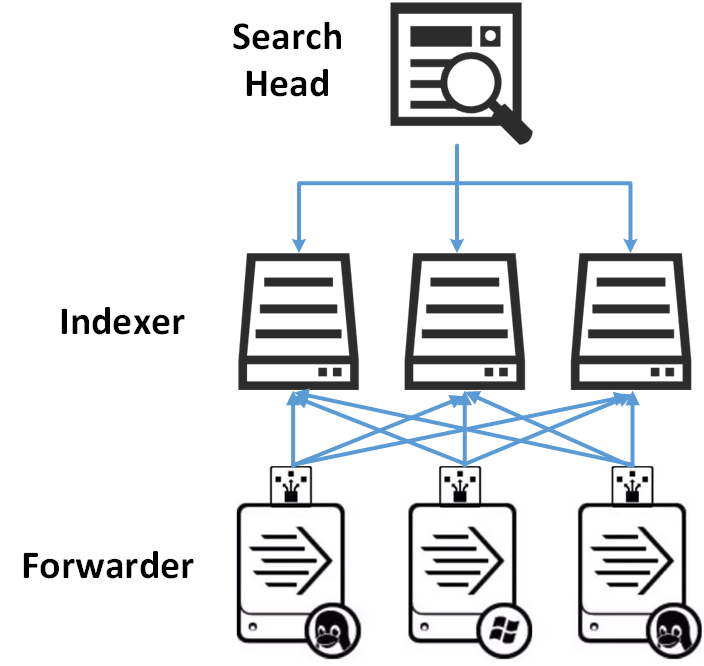
\includegraphics[scale = 0.55]{Figures/splunk.png}
    \end{generalfig}

    \subsubsection{数据图表应用场景概述}
    在运营商日常的网络管理工作中,会有各种各样的报表制作需求,从简单的每日流量统计情况、到每月网络整体情况总结,亦或是突发故障分析报告,都离不开数据的呈现与展示。但现阶段在部分运营商的报表制作
    呈现中,由于时间和技术的限制,往往还充斥着较为原始的数据罗列和单一的折线表现形式,这种表现形式除了制作者能对其中的含义能够快速清晰的了解,由于报表呈现展示的对象通常是不具备全面专业
    知识的管理者,这些信息对他们来说不够直观清晰,理解起来较为费劲,遇见突发状况时也不能对网络情况快速做出应对,导致客户感知较差,网络管理效率较低。因此,在日常报表制作中将数据转化成
    清晰直观恰当的图标形式会使得数据呈现效果大幅提升。

    不同的图表应用于不同的场景,清晰了解不同图表的优劣势会使得制作图表时能够更加得心应手,呈现思想也会清晰直观。常用的图表形式包括:柱状图、条形图、折线图、饼图,除此之外,还有较为新颖的
    数据地图、漏斗图、词云、散点图等。接下来就部分图表形式的使用场景进行简要概括:

    \begin{enumerate}
        \item {\bfseries 柱状图:\\}
        适用场景:适用场合是二维数据集(每个数据点包括两个值x和y),但只有一个维度需要比较,用于显示一段时间内的数据变化或显示各项之间的比较情况。适用于枚举的数据,比如地域之间的关系,数据没有必然的连续性。\\
        优势:柱状图利用柱子的高度,反映数据的差异,肉眼对高度差异很敏感。\\
        劣势:柱状图的局限在于只适用中小规模的数据集。
        \begin{generalfig}[htb]{柱状图}{fig:ZZT} 
            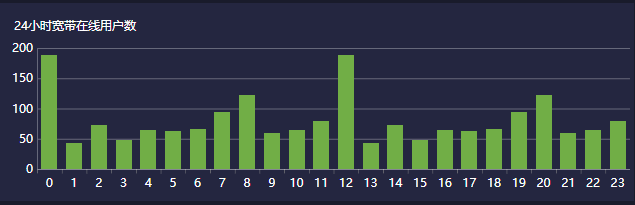
\includegraphics[width = \textwidth]{Figures/ZZT.png}
        \end{generalfig}
        \item {\bfseries 条形图:\\}
        适用场景:显示各个项目之间的比较情况,和柱状图类似的作用。\\
        优势:每个条都清晰表示数据,直观。\\
        \begin{generalfig}[htb]{条形图}{fig:TXT} 
            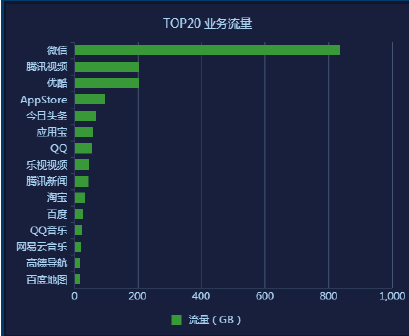
\includegraphics[scale = 1]{Figures/TXT.png}
        \end{generalfig}
        \item {\bfseries 折线图:\\}
        适用场景:折线图适合二维的大数据集,还适合多个二维数据集的比较。一般用来表示趋势的变化,横轴一般为日期字段。\\
        优势:容易反应出数据变化的趋势。\\ 
        \begin{generalfig}[htb]{折线图}{fig:ZXT} 
            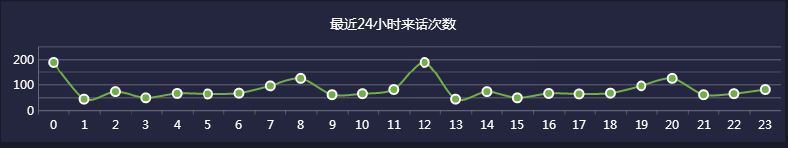
\includegraphics[width = \textwidth]{Figures/ZXT.png}
        \end{generalfig}
        \item {\bfseries 数据地图:\\}
        适用场景:适用于有空间位置的数据集,能够将事件与地理位置相关联。\\ 
        优劣势:特殊状况下使用,涉及行政区域。\\
        \begin{generalfig}[htb]{数据地图}{fig:SJDT} 
            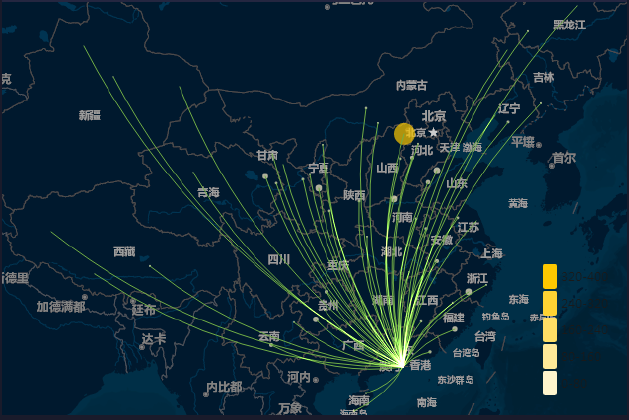
\includegraphics[width = \textwidth]{Figures/SJDT.png}
        \end{generalfig}
    \end{enumerate}

    

    
    

\end{document} 